\section{Experiment} \label{sec:experiment}

\subsection{Evaluation metric}

% While we training and compute loss function for backpropagation on generated ground-truth density map,

From the predicted density map, we acquired predicted count by integral the density map over the whole image (i.e., sum all pixel values in the predicted density map matrix). Then from the predicted count and annotated count, compute Mean Absolutately Error (MAE), Mean Square Error (MSE) 

\begin{equation}M A E=\frac{1}{N} \sum_{i=1}^{N}\left|C_{i}^{e t}-C_{i}^{g t}\right|\end{equation}

\begin{equation}M S E=\sqrt{\frac{1}{N} \sum_{i=1}^{N}\left(C_{i}^{e t}-C_{i}^{g t}\right)^{2}}\end{equation}

\subsection{ShanghaiTech} \label{sec:shb_result}
 
%% TODO: writer something about ShanghaiTech B 
%% ShanghaiTech B is medium - low density 


ShanghaiTech \cite{zhang2016single} is one of the most common benchmark datasets for crowd counting and more specific crowd density estimation. The dataset comes with the location of the heads annotated. Part A consists of images of dense crowd scenes, taken on the Internet, of variable format (black and white, color), variable size. Part B is low to medium crowd scenes taken from Shanghai with fixed resolution of 1024x786 in RGB color format. 

Table \ref{tab:experiment-result} show experiment result our proposed method comparing to C-CNN. Fig. \ref{fig:result-picture} shows the comparison result of both C-CNN (second row) and DCCNN (third row). Density maps generated by DCCNN are sharper and less background noise than of C-CNN.

% The increase in parameter size due to learnable affine parameters in batch normalization.  

% \begin{table}[htbp]
% \caption{\label{tab:experiment-result}  Experiment result}
% \begin{center}
% \begin{tabular}{|c|c|c|}
% \hline
% \textbf{}&\multicolumn{2}{|c|}{\textbf{ShanghaiTech B}}\\
% \hline
% \textbf{Model} & \textbf{\textit{MAE}}& \textbf{\textit{MSE}} \\
% \hline
% C-CNN \cite{9053780} & 14.9 & 22.1   \\
% \hline
% Ours & 12.2 & 21.9  \\
% \hline

% \end{tabular}

% \end{center}
% \end{table}


\begin{table}[htbp]
\caption{\label{tab:experiment-result}  Experiment result}
\begin{center}
\begin{tabular}{|c|c|c|c|c|}
\hline
\textbf{}&\multicolumn{2}{|c|}{\textbf{ShanghaiTech A}}&\multicolumn{2}{|c|}{\textbf{ShanghaiTech B}}\\
\hline
\textbf{Model} & \textbf{\textit{MAE}}& \textbf{\textit{MSE}} & \textbf{\textit{MAE}}& \textbf{\textit{MSE}} \\
\hline
C-CNN \cite{9053780} & 88.1 & 141.7  & 14.9 & 22.1   \\
\hline
Ours & 84.1 & 133.5 & 12.2 & 21.9  \\
\hline

\end{tabular}

\end{center}
\end{table}

\begin{figure}[htbp]
\centerline{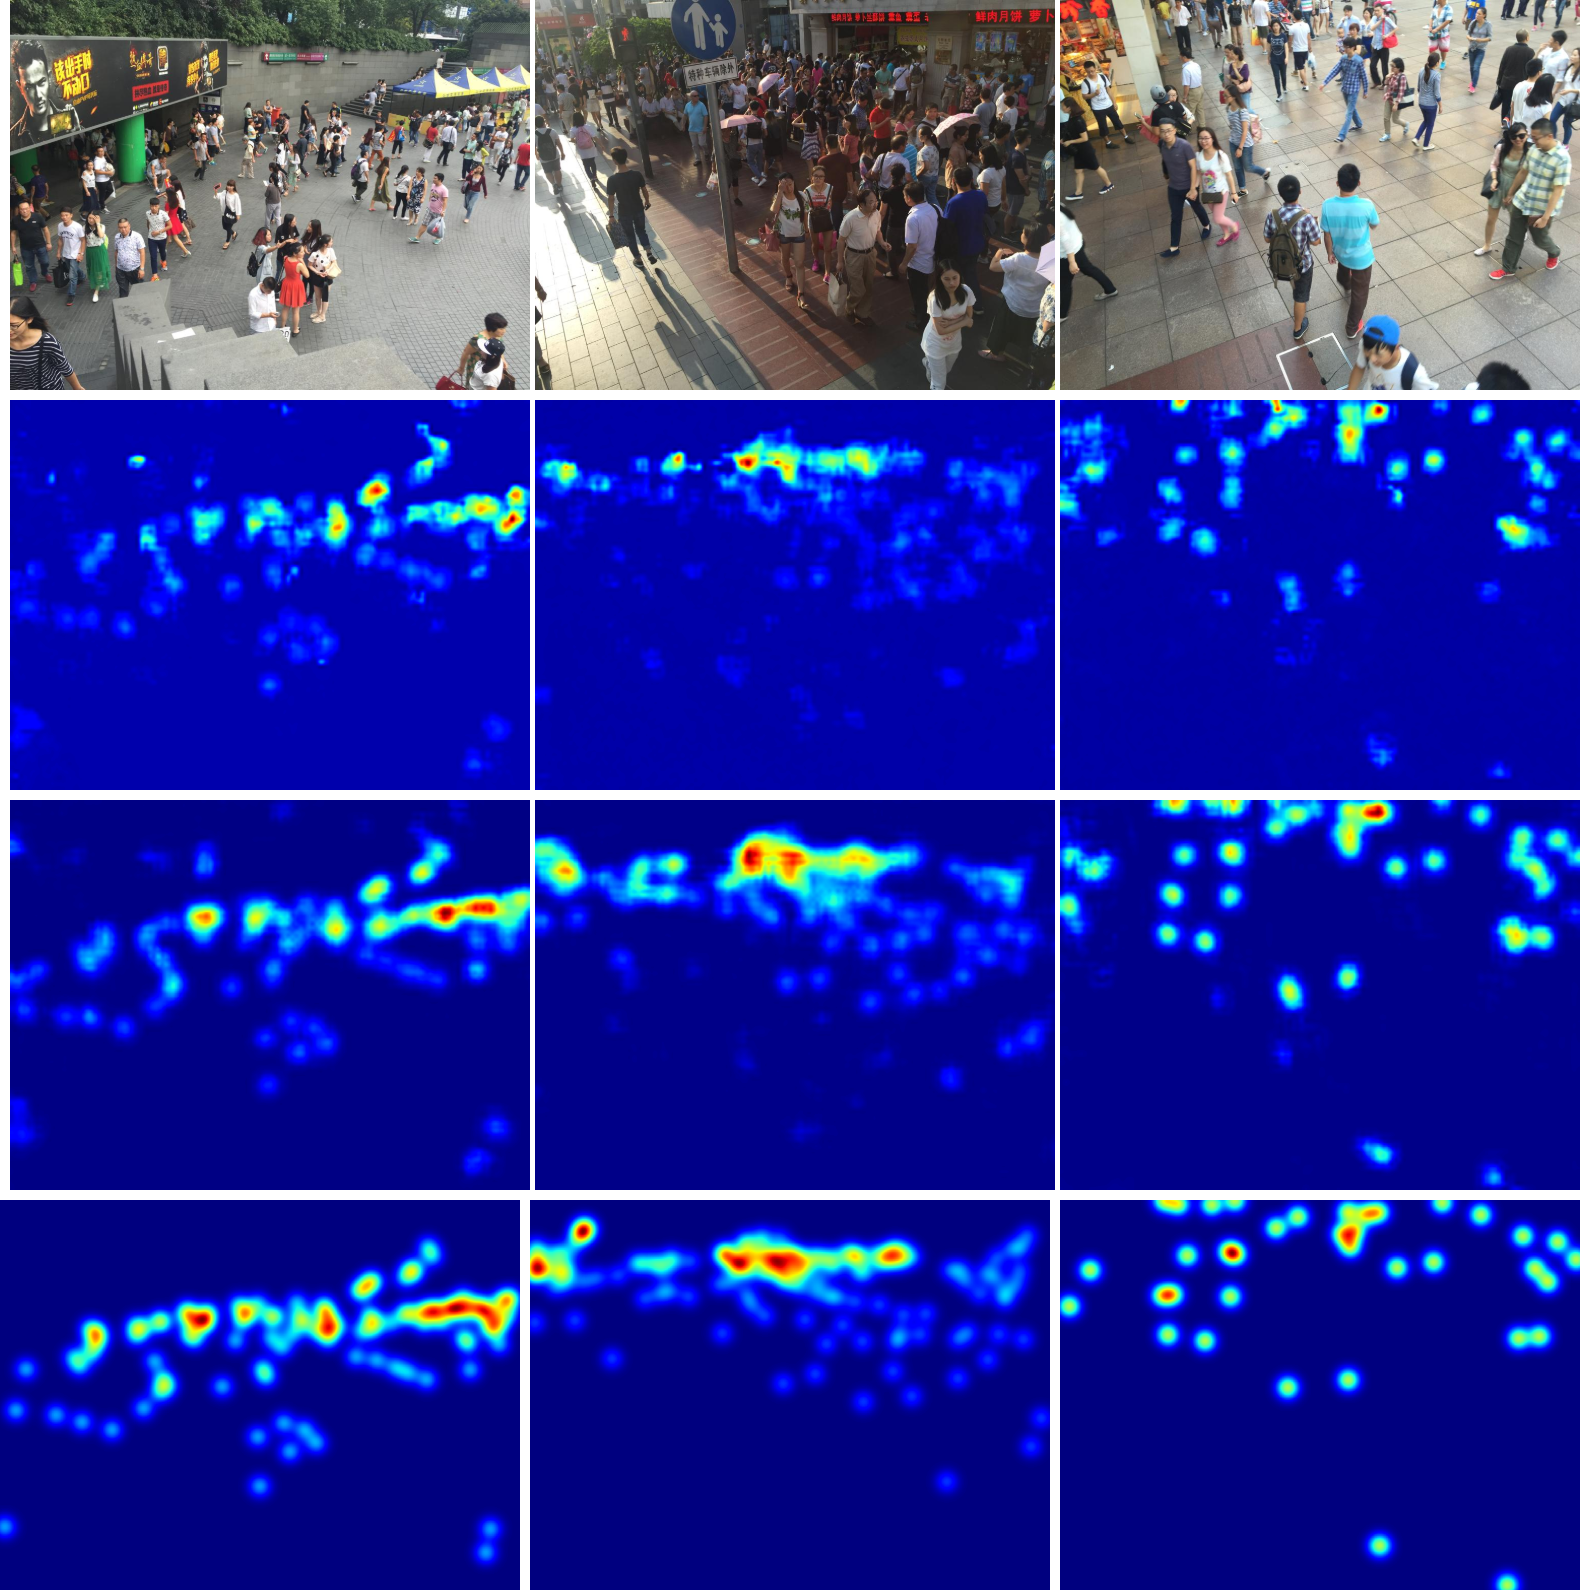
\includegraphics[width=0.4\textwidth]{Picture/result/result_ccnn_vs_bigtail.png}}
\caption{From top down: Original image, C-CNN \cite{9053780} estimation, DCCNN estimation, ground-truth density map, respectively.}
\label{fig:result-picture}
\end{figure}





% % benchmark FPS
% \begin{table}[htbp]
% \caption{\label{tab:benchmark}  Benchmark}
% \begin{center}
% \begin{tabular}{|c|c|c|}
% \hline
% \textbf{}&\multicolumn{2}{|c|}{\textbf{ShanghaiTech B}} \\
% \hline
% \textbf{Model} & \textbf{\textit{Average time (seconds)}}& \textbf{\textit{FPS}} \\
% \hline
% C-CNN (authors) &   & 104.16    \\
% \hline
% C-CNN (our implementation) & 7.15 &  44.5    \\
% \hline
% Ours & 6.95 & 45.7 \\
% \hline
% % \multicolumn{3}{l}{$^{\mathrm{a}}$ Parameter size in our implementation.}
% \end{tabular}

% \end{center}
% \end{table}

\subsection{Benchmark}

We run benchmark our re-implementation C-CNN \cite{9053780} and our proposed DCCNN on predefined ShanghaiTech B test set, total 318 test images, on the same hardware. Our benchmarks are run on a personal desktop with Intel Core i5-9400 CPU @ 2.90GHz x 6 and GeForce GTX 1070 Ti graphic card. Images are kept as their original size. Models are run on inference mode on a batch size of 1. We count the number of trainable parameters and measure total running time in second. Benchmark results are summarized in Table \ref{tab:benchmark-result}. Running times are averaged from multiple runs of the same setting. Unfortunately, we cannot reproduce C-CNN benchmark of original authors \cite{9053780} (104.16 FPS) due to hardware limitations. 

\begin{table}[htbp]
\caption{\label{tab:benchmark-result}  Benchmark}
\begin{center}
\begin{tabular}{|c|c|c|c|}
\hline
\textbf{}&\multicolumn{2}{|c|}{\textbf{ShanghaiTech B}}&\textbf{Parameter} \\
\cline{1-3}
\textbf{Model} & \textbf{\textit{ Time (seconds) }}& \textbf{\textit{FPS}}&\textbf{Size} \\
\hline
C-CNN (authors) \cite{9053780} &  &  104.16 & 0.07M \\
\hline
C-CNN$^{\mathrm{a}}$  & 6.95482 & 45.72 & 72509   \\
\hline
Ours &  7.15093 & 44.47 & 73009 \\
\hline
\multicolumn{4}{l}{$^{\mathrm{a}}$ Our re-implementation of C-CNN \cite{9053780}}
\end{tabular}

\end{center}
\end{table}

Comparing to C-CNN \cite{9053780}, our DCCNN requires more computing resources due to: 
\begin{itemize}
    \item Batch normalization: 500 trainable affine parameters, more computation.
    \item 2 layer of average pooling instead of max pooling: more computation. 
\end{itemize}

Despite the noticeable performance improvements of DCCNN, the additional resources required are negligible.